%Typeset with LuLaTex !!!!
\documentclass{article}

% Language setting
% Replace `english' with e.g. `spanish' to change the document language
\usepackage[english]{babel}
%\usepackage{CJKutf8}%pdflatex

%\usepackage{xeCJK}
%\setCJKmainfont{Noto Serif CJK JP}%fonts not found
%\setCJKsansfont{Noto Sans CJK JP}
%\setCJKmonofont{Noto Sans Mono CJK JP}

\usepackage{luatexja}

% Set page size and margins
% Replace `letterpaper' with `a4paper' for UK/EU standard size
\usepackage[letterpaper,top=1.5cm,bottom=1.6cm,left=2.5cm,right=2.5cm,marginparwidth=1.75cm]{geometry}

% Useful packages
\usepackage{graphicx}
\usepackage{enumitem}


%\title{Your Paper}
%\author{You}

\begin{document}
\pagenumbering{gobble}

%\section{Heike --- Principal Characters}


\vspace*{-0.4cm}
\begin{small}

    %\begin{compacthang}
    \begin{itemize}[
            label=,
            leftmargin=0em,
            itemindent=-2em,
            nosep,
        ]

        \item \textbf{Antoku, \textit{Emperor}}. Son of Emperor Takakura and Kenreimon’in; grandson of Kiyomori.

        \item \textbf{Atsumori, \textit{Taira}}. Son of Tsunemori; nephew of Kiyomori. Died at Ichi-no-tani.

        \item \textbf{Dainagon-no-suke}. Daughter of Gojō Major Counselor Kunitsuna; wife of Shigehira; one of Emperor Antoku’s nurses; lady-in-waiting to Kenreimon’in.

        \item \textbf{Go-Shirakawa, \textit{Retired Emperor}}. Son of Retired Emperor Toba and Tai-kenmon’in; exercised authority during reigns of Emperors Nijō, Rokujō, Takakura, Antoku, and Go-Toba. Nijo and Takakura were his sons; Rokujo, Antoku, and Go-Toba, his grandsons.

        \item \textbf{Jaro Kurando}, see Yukiie.

        \item \textbf{Kagetoki, \textit{Kajiwara}}. Trusted lieutenant of Yoritomo; figures in Heike mo-nogatari as provoking Yoritomo’s enmity toward Yoshitsune.

        \item \textbf{Kamakura Lord}, see Yoritomo.

        \item \textbf{Kanehira, \textit{Imai}}. Foster-brother of Kiso no Yoshinaka.

        \item \textbf{Kenreimon'in}. Daughter of Kiyomori and Nun of Second Rank; full sister of Munemori, Tomomori, and Shigehira; consort of Emperor Taka-kura; mother of Emperor Antoku. Taken prisoner at Dan-no-ura; died as a nun.

        \item \textbf{Kiso}, see Yoshinaka.

        \item \textbf{Kiyomori, \textit{Taira}}. Son of Tadamori; head of clan after father’s death; dominated court.

        \item \textbf{Koremori, \textit{Taira}}. Oldest son of Shigemori; committed suicide after taking religious vows.

        \item \textbf{Michimori, \textit{Taira}}. Son of Norimori; nephew of Kiyomori. Died at Ichi-no-tani.

        \item \textbf{Mochihito, \textit{Prince}}. Second son of Retired Emperor Go-Shirakawa; nominal leader of revolt against Taira in 1180. Called Prince Takakura.

        \item \textbf{Mongaku, \textit{monk}}. In Heike monogatari, incites Yoritomo to rebellion; later gains reprieve for Koremori’s son, Rokudai.

        \item \textbf{Munemori, \textit{Taira}}. Son of Kiyomori and Nun of Second Rank; clan head after father’s death; Palace Minister. Executed in 1185.

        \item \textbf{Narichika, \textit{Fujiwara}}. Close associate of Retired Emperor Go-Shirakawa; brother-in-law of Shigemori; father-in-law of Koremori. Executed for plotting revolt against Taira in 1177.

        \item \textbf{Naritsune, \textit{Fujiwara}}. Son of Narichika; exiled to Kikai-ga-shima.

        \item \textbf{Norimori, \textit{Taira}}. Son of Tadamori; brother of Kiyomori; father-in-law of Narichika’s son Naritsune. Died at Dan-no-ura.

        \item \textbf{Noritsune, \textit{Taira}}. Son of Norimori; nephew of Kiyomori. Depicted in Heike monogatari as a leading Taira commander.

        \item \textbf{Noriyori, \textit{Minamoto}}. Son of Yoshitomo; half-brother of Yoritomo. One of Yoritomo’s two principal commanders in the Genpei campaigns.

        \item \textbf{Nun of Second Rank. \textit{Taira} no Shishi (Tokiko)}, principal wife of Kiyomori and mother of Munemori, Tomomori, Shigehira, and Kenreimon’in. Died at Dan-no-ura.

              \vspace{0.2cm} %blank item for page fold

        \item \textbf{Rokudai, \textit{Taira}}. Son of Koremori; grandson of Shigemori.

        \item \textbf{Shigehira, \textit{Taira}}. Son of Kiyomori and Nun of Second Rank. Important Taira commander; captured at Ichi-no-tani and later executed.

        \item \textbf{Shigemori, \textit{Taira}}. Oldest son and heir of Kiyomori, whom he predeceased. Palace Minister.

        \item \textbf{Sotsu-no-suke}. Wife of Tokitada; one of Emperor Antoku’s nurses.

        \item \textbf{Sukemori, \textit{Taira}}. Second son of Shigemori. Died at Dan-no-ura.

        \item \textbf{Tadamori, \textit{Taira}}. Clan head; father of Kiyomori.

        \item \textbf{Tadanori, \textit{Taira}}. Son of Tadamori; brother of Kiyomori. Known as a poet. Died at Ichi-no-tani.

        \item \textbf{Takakura, \textit{Emperor}}. Son of Retired Emperor Go-Shirakawa and Kenshun-mon’in; nephew of Tokitada. Married to Kenreimon’in; father of Emperor Antoku.

        \item \textbf{Takakura, \textit{Prince}}, see Mochihito.

        \item \textbf{Tokimasa, \textit{Hojo}}. Yoritomo’s deputy in the capital after the breach with Yoshitsune.

        \item \textbf{Tokitada, \textit{Taira}}. Member of a branch family. Brother of Kenshunmon’in; uncle of Emperor Takakura; brother of Nun of Second Rank. Major Counselor.

        \item \textbf{Tomomori, \textit{Taira}}. Son of Kiyomori and Nun of Second Rank. Figures in Heike monogatari as a military leader. Died at Dan-no-ura. Tsunemasa, Taira. Oldest son of Tsunemori; nephew of Kiyomori. Known as a poet and musician. Died at Ichi-no-tani.

        \item \textbf{Tsunemori, \textit{Taira}}. Brother of Kiyomori; Consultant.

        \item \textbf{Yorimasa, \textit{Minamoto}}. Distant relative of Yoritomo; military leader in revolt of Prince Mochihito.

        \item \textbf{Yorimori, \textit{Taira}}. Half-brother of Kiyomori; son of Yoritomo’s benefactor, Lady Ike. Provisional Major Counselor.

        \item \textbf{Yoritomo, \textit{Minamoto}}. Son and eventual heir of Yoshitomo; eastern hegemon; founder of Kamakura Shogunate after victory in Genpei War. Yoshimori, see Yukiie.

        \item \textbf{Yoshinaka, \textit{Minamoto}}. Son of Yoshikata; cousin of Yoritomo. Leader of northern anti-Taira forces; killed in battle against Noriyori’s army.

        \item \textbf{Yoshinori, \textit{Minamoto}}. Son of Tameyoshi; brother of Yukiie; uncle of Yori-tomo. Military figure; sided first with Yoritomo, later with Yoshinaka.

        \item \textbf{Yoshitsune, \textit{Minamoto}}. Son of Yoshitomo; younger half-brother of Yoritomo. As one of Yoritomo’s two principal commanders, won pivotal victories in the Genpei campaigns. Later hounded by forces of the jealous Yoritomo.

        \item \textbf{Yukiie, \textit{Minamoto}}. Son of Tameyoshi; uncle of Yoritomo. Known at first as Yoshimori. Military leader; allied successively with Yoritomo, Yoshinaka, and Yoshitsune.

    \end{itemize}
    %\end{compacthang}

\end{small}

%page break for taira and imperial family trees
\clearpage

\begin{figure}
    \setlength\lineskip{-0.5in}
    \makebox[\textwidth][c]{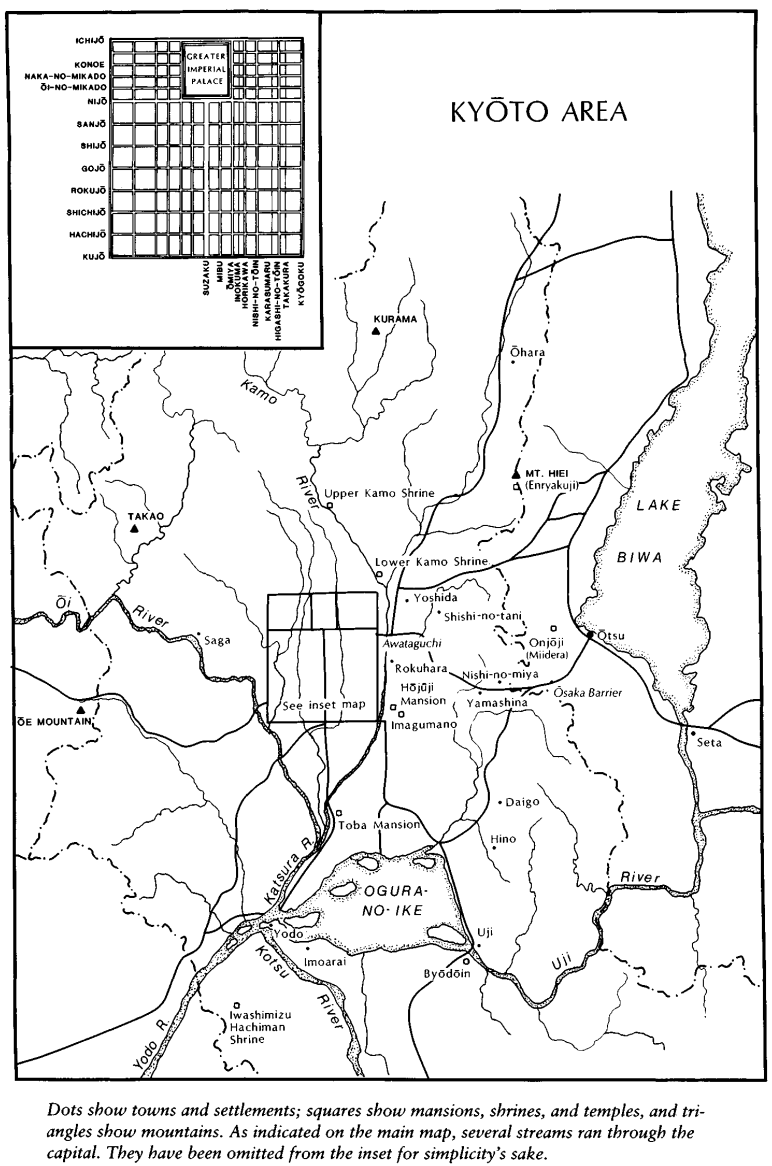
\includegraphics[angle=90,origin=c,width=1.2\linewidth]{heike-map-kyoto.png}}%

    \makebox[\textwidth][c]{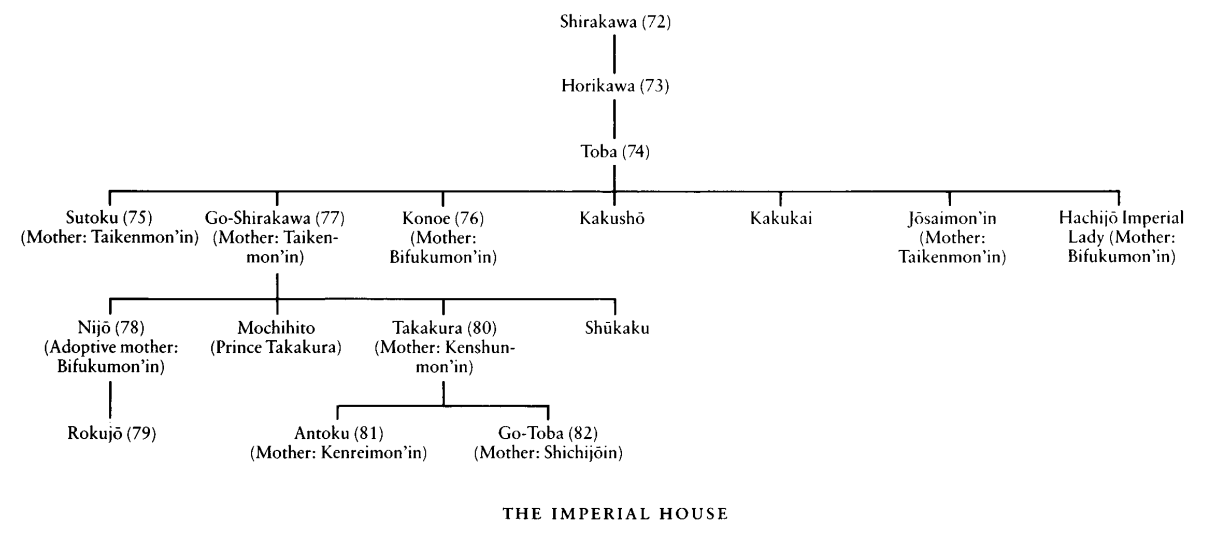
\includegraphics[width=1.2\textwidth]{heike-tree-imperial.png}}%
    %\caption{Caption}
    %\label{fig:key}
\end{figure}

%page break for kyoto map and miniamoto family tree
\clearpage


\begin{figure}
    \vspace*{-1.0cm}
    \setlength\lineskip{-1.0in}
    %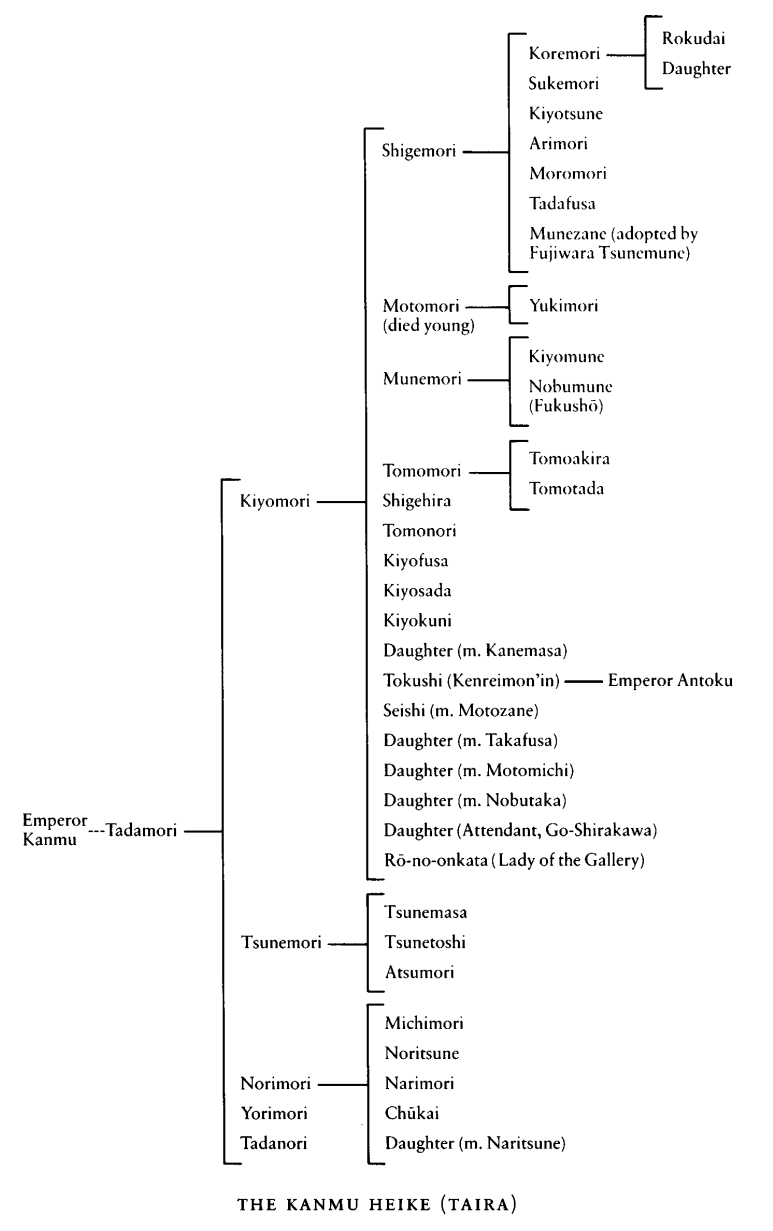
\includegraphics[angle=90,origin=c,width=1.2\linewidth]{heike-tree-taira.png}
    \makebox[\textwidth][c]{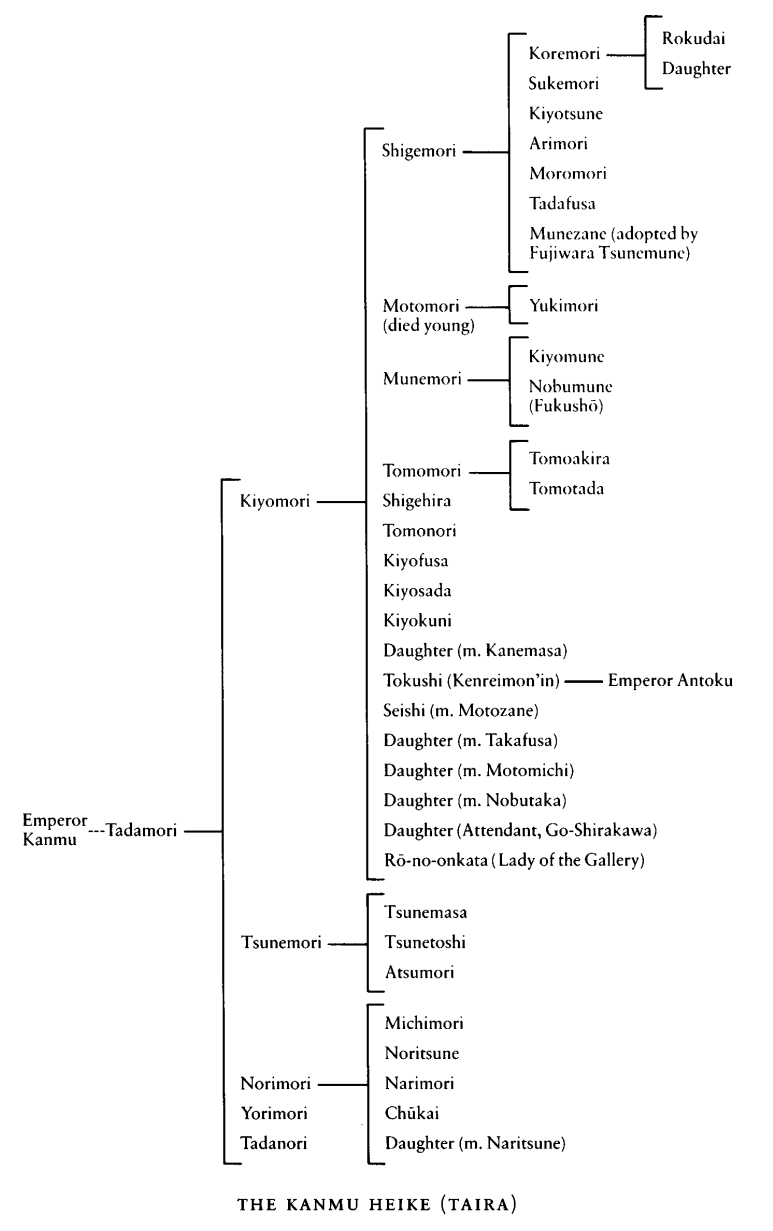
\includegraphics[angle=90,origin=c,width=1.2\linewidth]{heike-tree-taira.png}}%

    \begin{minipage}{0.6\textwidth}
        \hspace*{-1.75cm}
        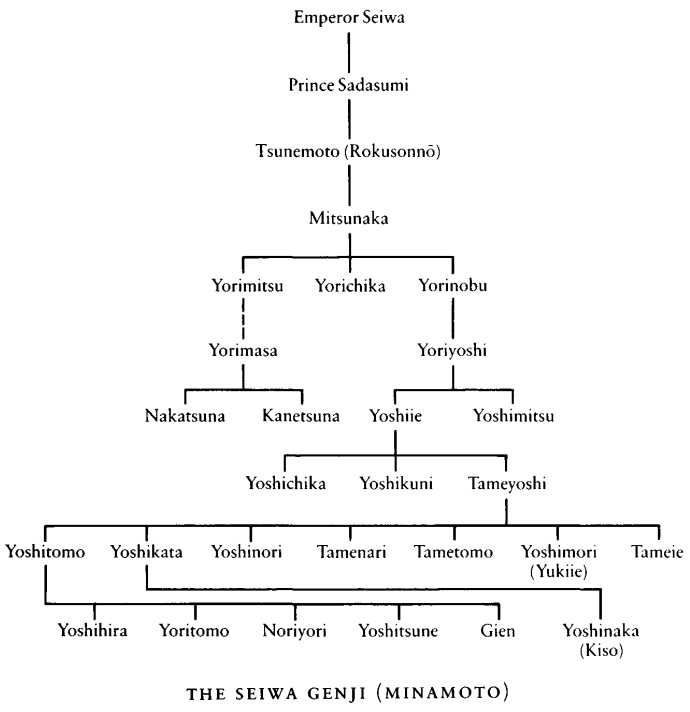
\includegraphics[height=4.5in]{heike-tree-minamoto.png}
        %\caption{second}
    \end{minipage}
    \begin{minipage}{0.4\textwidth}
        1\textsuperscript{st}--11\textsuperscript{th} sons: Tarō, Jiro, Saburō, Shirō, Gorō, Rokurō,Shichirō, Hachirō, Kurō, Jurō, and Jūichirō

        \vspace{1em}

        There were nine major designations for subjects,
        ranging in descending order of importance from
        Senior 1\textsuperscript{st} through
        Junior 8\textsuperscript{th} Lower
        to Lesser Initial Lower.
        Ranks 1--3 had two subdivisions each, Sr. and Jr.;
        and ranks 4--8 had four subdivisions each, Sr. Upper, Sr. Lower, Jr.
        Upper, and Jr. Lower.
        The two Initial ranks, Greater and Lesser, were also subdivided into Upper and Lower.

        \vspace{1em}

        Heike (平家) refers to the Taira (平), hei being the on'yomi reading of the first kanji and "ke" (家) meaning "family". However, in the term "the Genpei War" "hei" is read as "pei" and the "gen" (源) is the first kanji in "Genji" the alternative name for the Minamoto clan.

    \end{minipage}
\end{figure}





%page break for two part map of japan
\clearpage


% two part map of japan
\begin{figure}
    \setlength\lineskip{5pt}
    \makebox[\textwidth][c]{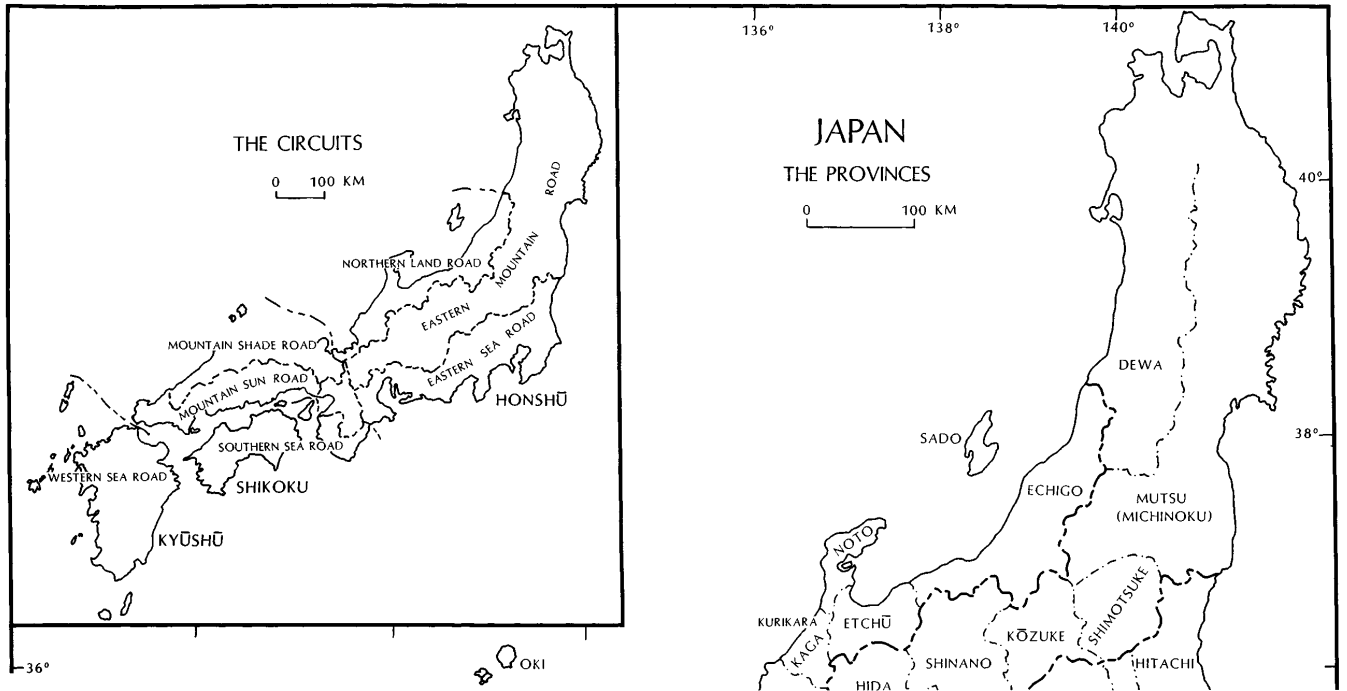
\includegraphics[width=1.2\textwidth]{heike-map-japan-top.png}}%

    \makebox[\textwidth][c]{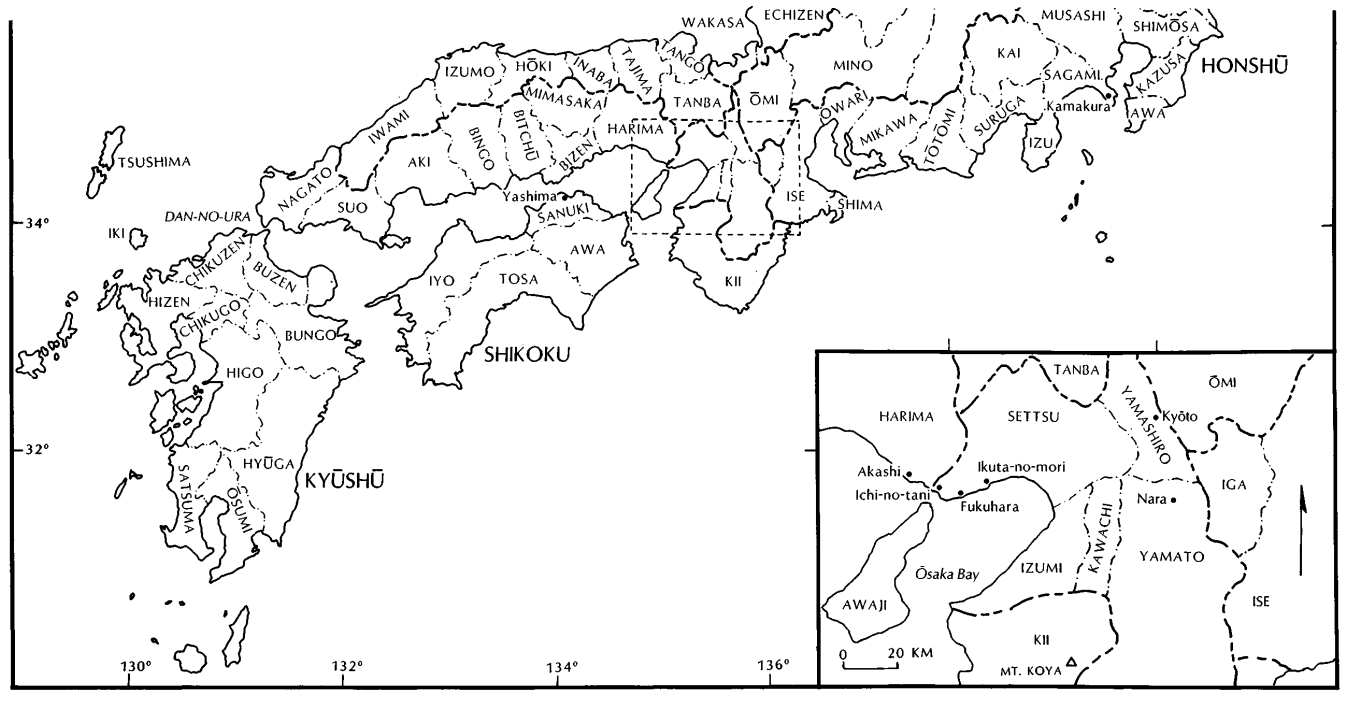
\includegraphics[width=1.2\textwidth]{heike-map-japan-bottom.png}}%
\end{figure}



%%page break for one part map of japan
%\clearpage

%\begin{figure}
%  \makebox[\textwidth][c]{\includegraphics[width=1.25\textwidth]{heike-map-japan.png}}%
%\end{figure}


\end{document}
